\documentclass{beamer}


\usepackage[utf8]{inputenc} 
\usepackage[T1]{fontenc}
\usepackage{lmodern}
\usepackage{graphicx}
\usepackage[french]{babel}

\usetheme{Warsaw}

\addtobeamertemplate{navigation symbols}{\usebeamerfont{footline}%
	\usebeamercolor[fg]{footline}%
	\hspace{1em}%
	\insertframenumber/\inserttotalframenumber}

\begin{document}

\AtBeginSection[]{
	
	\begin{frame}
	
	\frametitle{Sommaire}
	
	\tableofcontents[currentsection]
	
	\end{frame} 

}


\title[Plateforme d'acquisition multiflux TV Web]{Plateforme d'acquisition et de formatage temps réel multiflux TV Web}
\subtitle{Première soutenance de PR\&D}
\author{Romain ROUSSEAU}
\institute{Polytech Tours}
\date{\today}

\begin{frame}
	
	\maketitle
	
\end{frame}



\section*{Introduction}


\begin{frame}

\frametitle{Introduction}

Projet Recherche \& Développement consacré à l'étude et à la mise en place d'une plateforme d'acquisition de flux de TV Web.

Initié par Jordan NICOT, ancien élève de Polytech Tours, qui a effectué son projet libre à ce sujet.

\end{frame}


\begin{frame}

\frametitle{Sommaire}

\tableofcontents


\end{frame}


%------------------------

\section{Contexte}

\subsection{Contexte général}

\begin{frame}	

\frametitle{Contexte général}

La diffusion de contenu audio et vidéo représente plus de 75\% du trafic actuel sur Internet.

Atteindra plus de 80\% à l'horizon 2021. (Source Cisco, 2017)

\end{frame}

\begin{frame}	

\frametitle{Contexte général}

Les grands groupes de l'audio-visuel disposent déjà de plateforme proposant du contenu en direct.

\begin{center}

\includegraphics[scale=0.65]{Rapport_PR&D/images/exemple_sites}
\end{center}

\end{frame}


\begin{frame}	

\frametitle{Contexte général}

L'analyse temps réel de flux fait l'objet d'enjeux majeurs et peut être utilisé dans de nombreux domaines.

\begin{itemize}
	\item La propriété intellectuelle
	\item La recommandation de vidéo
	\item Le contrôle des vidéos, pour la publicité par exemple
	\item et bien d'autres...
\end{itemize}

\end{frame}


\subsection{Objectifs}

\begin{frame}	

\frametitle{Objectifs}

L'objectif, à la fin du projet, est d'avoir une plateforme d'acquisition de flux en ligne qui peut afficher les différents flux sélectionnés.

Par la suite, afficher différentes informations concernant les flux affichés (nombre d'images par seconde, débit, etc.).


\end{frame}


%-------------------------------

\section{\'{E}tat de l'art}

\subsection{Principe général du streaming}


\begin{frame}	
\frametitle{Principe général du \textit{streaming}}

Le terme \textit{Streaming} est tiré de l'anglais \textit{stream} signifiant flot ou courant en français. Ce terme désigne aujourd'hui la diffusion en continu sur Internet de contenus audio-visuels.

Nous nous intéresserons uniquement aux flux vidéos par la suite (bien que les autres flux fonctionnent de manière similaire).


\end{frame}

\begin{frame}	
\frametitle{Lecture progressive vs Lecture en continu}

Les données sont mises à disposition sur un serveur et pour récupérer ses informations, le client envoie une requête et récupère le flux envoyé.

\begin{description}
	\item[Lecture progressive] La vidéo est chargée, les données sont mises en cache par le client et la vidéo commence lorsqu'il y a assez de données en cache pour la commencer. On la retrouve pour le visionnage de vidéos Youtube par exemple.
	\item[Lecture en continu] Le contenu est diffusé au même rythme que la lecture. Le fichier envoyé par le serveur n'a pas de début et de fin définis.
\end{description}


\end{frame}


\subsection{Les protocoles de communication}

\begin{frame}	
\frametitle{Les protocoles de communication}

Il existe de nombreux protocoles pour transférer des flux de données en direct.

\begin{itemize}
	\item HTTP
	\item RTSP et RTSP 2.0
	\item RTMP
	\item MPEG-DASH, HLS, HDS, etc.
\end{itemize}

\end{frame}

\begin{frame}	
\frametitle{HTTP}

Protocole de communication réputé, standardisé en 1996, à la base de l'Internet moderne.

C'est le protocole le plus utilisé pour envoyer des données média à travers Internet, et d'autant plus avec l'arrivée et la démocratisation de HTML5.

\end{frame}

\begin{frame}	
\frametitle{RTSP et RTSP 2.0}

RTSP est un protocole pionnier de la diffusion en continu. Il a été standardisé en 1998.
Utilise les protocoles de transport RTP et RTCP pour transmettre les données.

Devenu obsolète et remplacé par sa version 2.0 en 2016.

\end{frame}

\begin{frame}	
\frametitle{RTMP}

Protocole propriétaire développé par Macromedia (racheté par Adobe Systems) en 2005, il était le protocole dominant lors des années 2000. 

Utilise le client \textit{Flash Player} pour fonctionner.

Aujourd'hui au bord de la disparition avec l'abandon de \textit{Flash Player}.

\end{frame}


\begin{frame}	
\frametitle{MPEG-DASH, HLS et les nouveaux protocoles basés sur HTTP}

MPEG-DASH, développé par le groupe MPEG, fait partie des protocoles les plus populaires. Il est basé sur HTTP et est standardisé en 2012. 

Dans le même style, on a HLS, développé par Apple, utilisé sur les plateformes comme \textit{MyCanal}.

Ces protocoles gèrent le \textit{streaming} adaptatif.

\end{frame}

\subsection{Les librairies et outils d'acquisition}


\begin{frame}	
\frametitle{Les outils et librairies d'acquisition}

Il existe de nombreux outils et librairies permettant d'acquérir et de traiter des flux TV. Nous allons en voir deux: FFMPEG et VLC.

\end{frame}

\begin{frame}	
\frametitle{FFMPEG}

\begin{figure}
	
\includegraphics[scale=0.5]{Rapport_PR&D/images/ffmpeg}
\end{figure}

Ensemble de logiciels pour la gestion multimédia. Composé de 4 logiciels principaux: 

\begin{description}
	\item[ffmpeg] outil pour convertir des fichiers multimédia
	\item[ffserver] serveur pour la diffusion en ligne
	\item[ffplay] lecteur multimédia
	\item[ffprobe] outil d'analyse de flux multimédia.
\end{description}


Propose également des librairies à destination des développeurs.

\end{frame}

\begin{frame}	
\frametitle{libVLC}

\begin{figure}
	
\includegraphics[scale=0.25]{Rapport_PR&D/images/vlc-media-player-logo}
	\caption{Logo de la VideoLAN Organization}
\end{figure}

Librairie initiée par la \textit{VideoLAN Organization}, qui est à l'origine du lecteur multimédia VLC.


\end{frame}


\section{Description Générale}

\subsection{Environnement}

\begin{frame}
\frametitle{Environnement du projet}

Ce projet sera testé sur les salles machines de l'école et branché sur le réseau de l'université.

\begin{figure}
	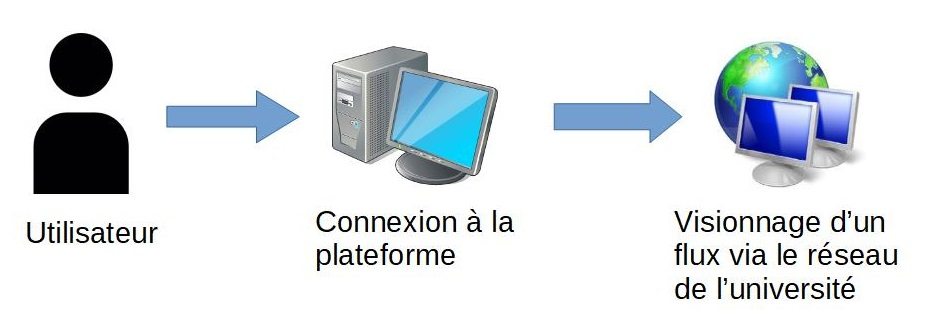
\includegraphics[scale=0.5]{Rapport_PR&D/images/environnement}
	\caption{Schéma de l'environnement du projet}
\end{figure}

\end{frame}


\subsection{Fonctionnalités du système}

\begin{frame}	
\frametitle{Fonctionnalités du système}
	
\begin{figure}
	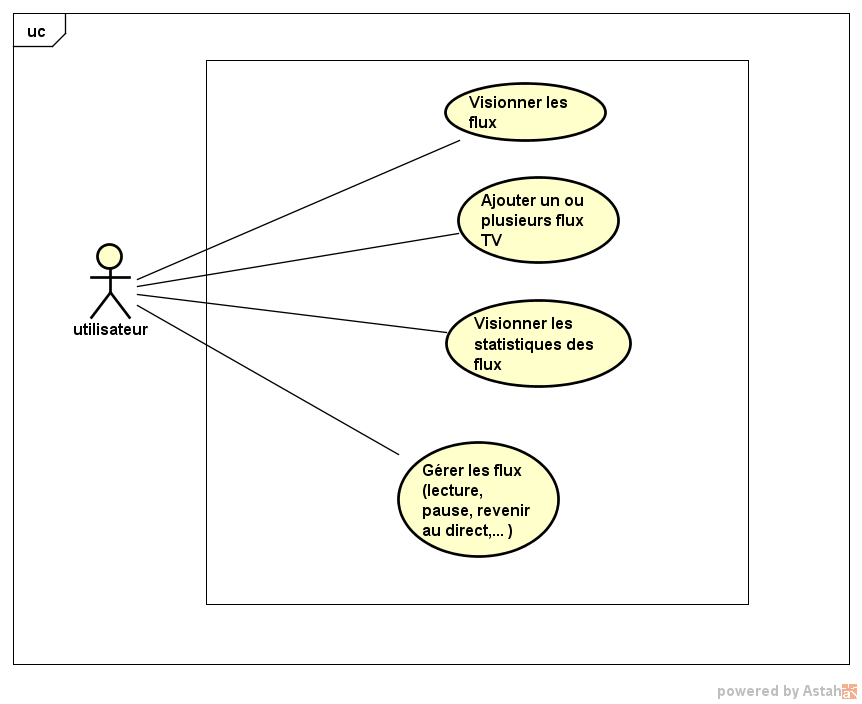
\includegraphics[scale=0.3]{Rapport_PR&D/images/UseCase}
	\caption{Diagramme de cas d'utilisation}
\end{figure}
	
\end{frame}


\subsection{Structure générale}

\begin{frame}	
\frametitle{Structure générale}

\begin{figure}
	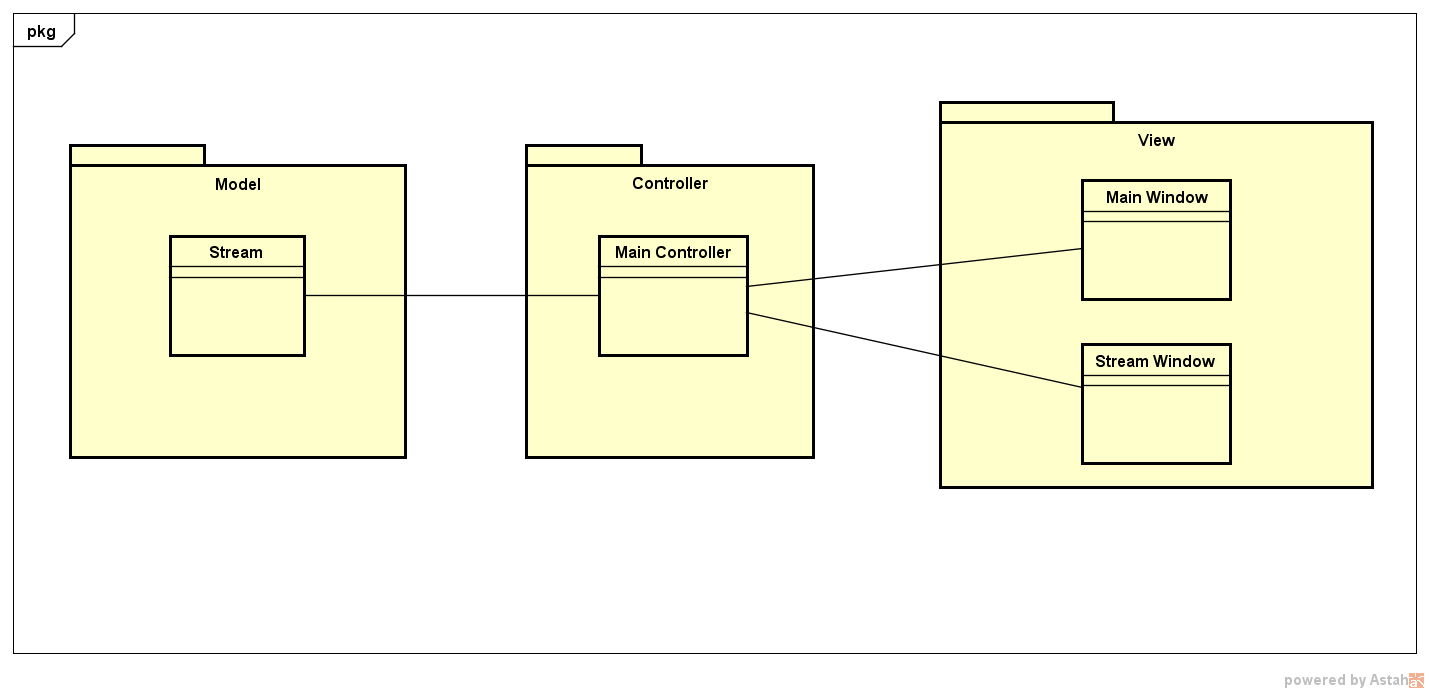
\includegraphics[scale=0.28]{Rapport_PR&D/images/ClassDiagram}
	\caption{Diagramme de structure}
\end{figure}

\end{frame}

\begin{frame}	

\begin{figure}
	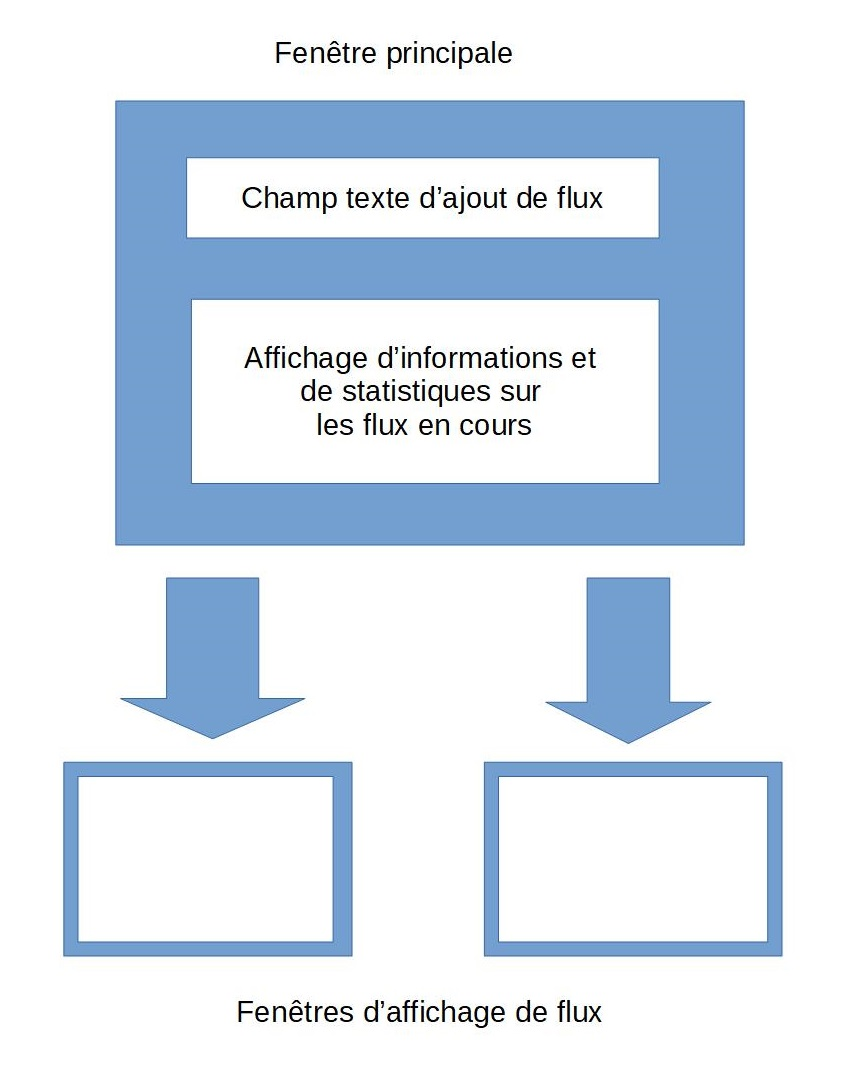
\includegraphics[scale=0.25]{Rapport_PR&D/images/ihm}
	\caption{Schéma de l'affichage}
\end{figure}

\end{frame}


\section*{Bilan et conclusion}

\begin{frame}	
\frametitle{Bilan et conclusion}


Nous avons une idée de l'architecture et de la mise en place, mais un problème reste en suspens: où et comment récupérer les flux TV ? 


Conception détaillée prévue mi-janvier, et premier livrable prévu fin-février au plus tard.



\end{frame}



\end{document}